\chapter{Implementación con CI}
  El objetivo de este práctico es armar y probar un decodificador BCD a 7 segmentos en un entorno de laboratorio
  reducido (minilab). El decodificador BCD a 7 segmentos (CD4511) es un circuito electrónico que toma una entrada de 4
  bits en formato BCD (Binary Coded Decimal) y la convierte en una salida correspondiente para mostrar un número decimal
  en un display de 7 segmentos.

  El circuito integrado CD4511 implementa una serie de entradas de control que permiten generar estados fuera del codigo
  BCD que son de utilidad. En la hoja de datos se especifican 3 entradas de control:
  \begin{itemize}
    \item \textbf{Lamp Test ($\overline{LT}$):} Traducido como "Prueba de Lampara", ignora el estado de la entrada BCD y pone todos
    los segmentos del LCD a VCC. Cuando esta entrada de control esta en estado logico bajo (0), el CI hace la prueba de
    lampara.
    \item \textbf{Blanking ($\overline{BL}$):} Traducido como "Blanqueo", ignora el estado de la entrada BCD y pone
    todos los segmentos del LCD a GND. Cuando esta entrada de control esta en estado logico bajo (0), el CI apaga el
    display de 7 segmentos.
    \item \textbf{Latch Enable ($\overline{LE}$):} Traducido como "Activar retencion", ignora el estado de la entrada
    BCD y deja fijo el estado de los segmentos del display como estaban antes de activar la retencion. Cuando esta
    entrada de control esta en estado logico bajo (0), el CI hace que la salida del display dependa del codigo BCD en
    las entradas. Cuando esta en estado logico alto (1), fija la salida del display e ignora el codigo BCD en la
    entrada.
  \end{itemize}

  Es importante destacar que estos estados especiales, tienen precedencia por sobre las entradas BCD. El orden en el que
  se presentaron las entradas de control, es el mismo en el que preceden, lo que significa que la entrada
  $\overline{LT}$ tiene precedencia por sobre $\overline{BL}$, que tiene precedencia por sobre $\overline{LE}$.

  Cabe destacar tambien, que segun la tabla de verdad provista en la hoja de datos, si la entrada BCD esta fuera del
  rango de 0 a 9 (en decimal), el CI dejara el display apagado, como forma de indicar que el numero BCD esta fuera de
  rango.

  \section{Implementacion en Protoboard}
    Puede revisar la seccion \ref{annex:schematic} para ver el esquematico del circuito que se puede ver en la figura
    \ref{fig:proto-cd4511}.

    Para la conexion entre el CI y el display de 7 segmentos, es necesario colocar resistencias
    limitadoras de corriente en serie. En caso de no colocar resistencias limitadoras en cada segmento, existe la
    posibilidad de dañar ambos, el display y el CI. Esto se debe a que por segmento, se requieren mas o menos $5mA$, y el
    CI, por segmento puede entregar hasta $20mA$ por pin, pero no mas de $50mA$ en simultaneo (segun hoja de datos).
    Por eso, se incluyeron resistencias de $470\Omega$ en serie para limitar la corriente a $10mA$ maximo por segmento.

    \begin{figure}[!ht]
      \centering
      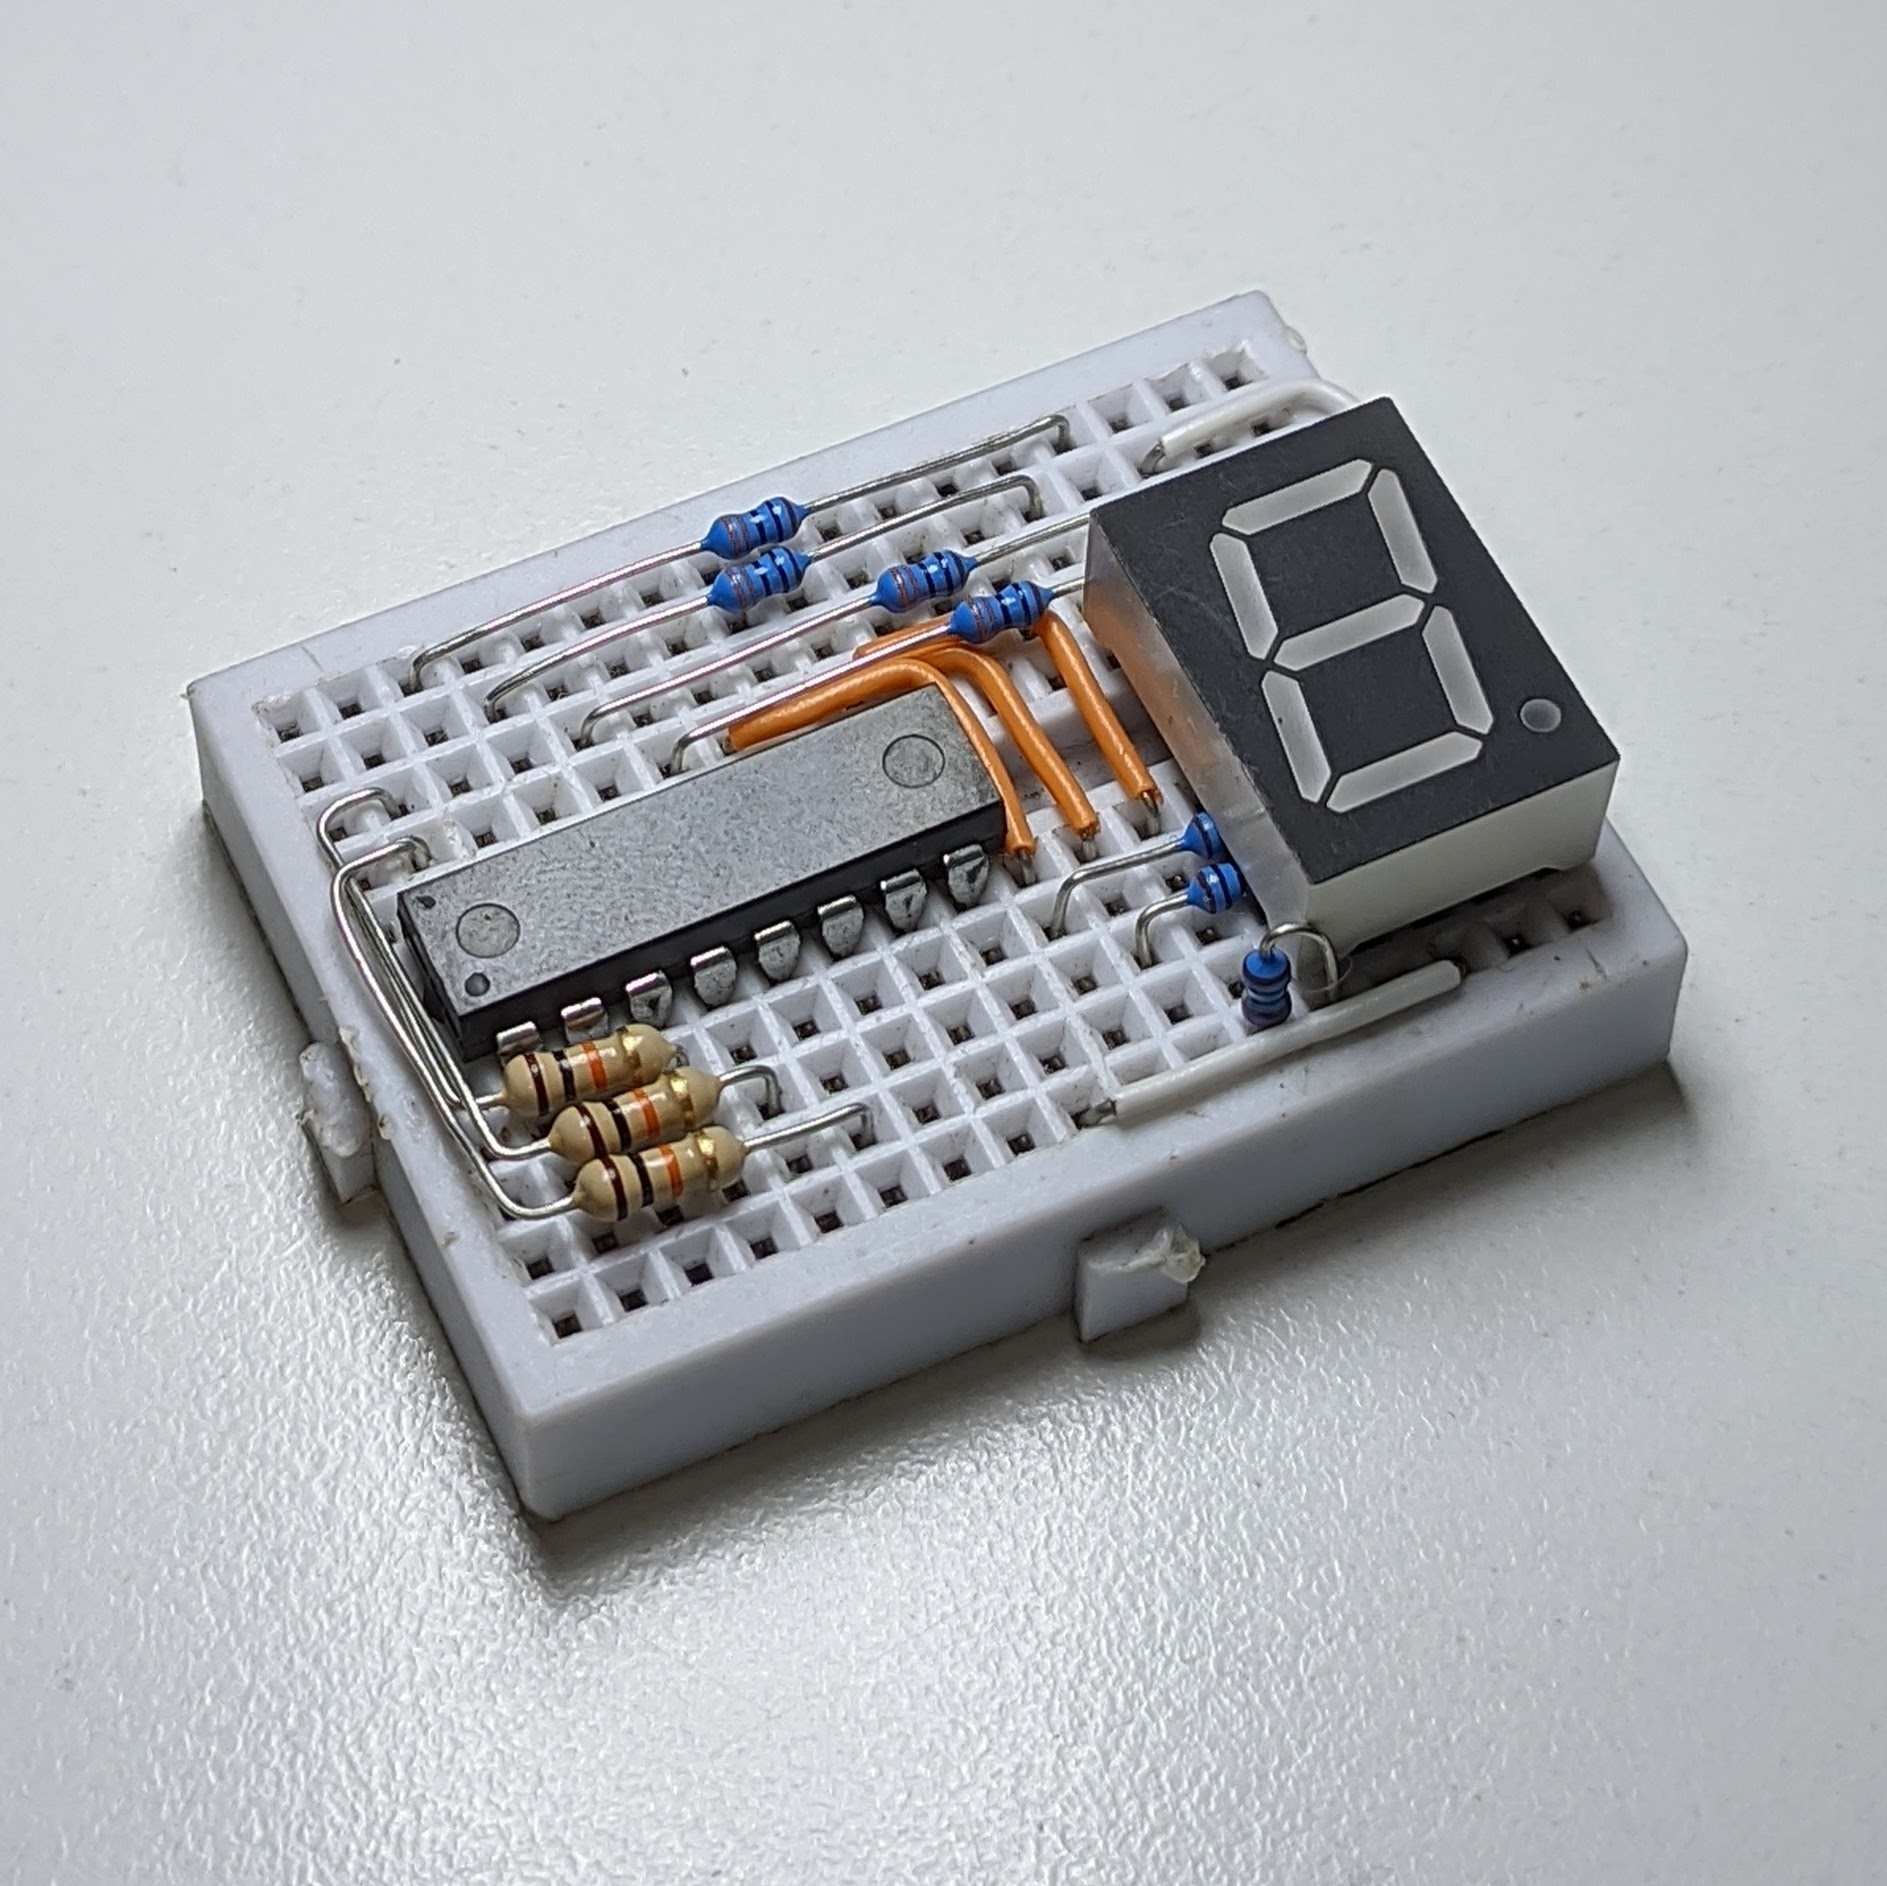
\includegraphics[width=0.8\textwidth]{pictures/cd4511-proto.jpg}
      \caption{circuito implementado en una protoboard.}
      \label{fig:proto-cd4511}
    \end{figure}
